\section{Introduction}

Cloud computing has marked significant developments and possibilities in the industry. It focuses on offering services for the different needs of the modern society.


There are three categories of cloud computing services namely, Software as a Service (SaaS), Platform as a Service (PaaS) and Infrastructure as a Service (IaaS). Organizations provide SaaS depending on the demand. Google Apps is one example of SaaS that can be used to manage email and create documents, etc. PaaS offers developers a platform where they can build and deploy applications. IaaS provides storage, servers and clusters. These tools are primarily created to serve computational needs \cite {Ahuja2012}. A cloud computing platform dynamically allocates, configures, reconfigures and deallocates servers as requested or on demand. This approach ensures the elasticity of cloud computing \cite {Brandic2011}.


Most scientific applications require high performance computing (HPC) which needs CPU intensive computations and large data storage. To be able to host such applications, several computers interconnected in a network such as clusters are needed. This makes scientific computing very costly in terms of hardware infrastructure investment. With the advancement in cloud computing, these scientific applications  can be deployed in the cloud without worrying about hardware costs and maintenance \cite {Ahuja2012}. However, studies have shown that network transmission delay is the major drawback in deploying HPC applications in the cloud\cite {Brandic2011}. 

Peak-Two Cloud (P2C) is a private cloud based on OpenStack designed for research in deploying HPC applications in the cloud\cite {Hermocilla2014}. One of the features introduced by P2C is vCluster. vCluster is a tool that enables a user to deploy a working (Message Passing Interface) cluster on demand and to terminate it after use. P2C has been used by researchers in various fields including bioinformatics, quantum chemistry, and molecular dynamics. These researchers belong to different research groups who have little or no investment in HPC infrastructure due to limited funding but requires heavy computing resources for their research. vCluster, however, is a command line application which make it difficult for non-technical users (physicists, chemists, and biologists) to use. A more user-friendly interface is needed in order to enable scientists to focus more on their science rather than on learning and using the command  line.

Presented in this paper is SkyLab\footnote{https://github.com/vincentpaul12/SkyLab}, a workflow web application on top of vCluster that addresses the concern above. Specifically, SkyLab will  

\begin{enumerate}
	\item allow users to execute HPC tools via web interface; 
	\item enable developers to easily extend it to support additional HPC tools;
	\item enable users to share their instantiated clusters; and
	\item support displaying of results using third party tools.
\end{enumerate}
   
The following are the tools that are currently supported by SkyLab. These are commonly used by collaborators from different research groups.

\begin{itemize}
    	\item \textit{AutoDock} - A software used to simulate protein-ligand docking\cite{morris2009autodock4}.

        \item \textit{AutoDock Vina} - A software similar to AutoDock 4 but on the average, it provides faster and more accurate computations \cite{JCC:JCC21334}. 
            
		\item \textit{DOCK} - Used to predict the small molecule-target interactions    \cite{lang2009dock}.
            
      	\item \textit{Quantum ESPRESSO} - An integrated software suite of tools for ab-initio molecular dynamics (MD) simulations and electronic structure calculations\cite{QE-2009}.

  		\item \textit{GAMESS} - Used for ab initio molecular quantum chemistry  \cite{1993gamess}.
            
 	    \item \textit{Ray} - Uses parallel genome assemblies for parallel DNA sequencing \cite{boisvert_ray_2012}.
 	    
 	    \item \textit{Impi} - MPI implementation of some image processing routines \cite{trajano2010}. 

\end{itemize}   

The use case on which SkyLab was designed is shown in Figure ~\ref{fig:usecase}. Users must first create a cluster then activate the desired tool to use.
      
\section{Design and Implementation}

SkyLab is implemented as a web application (using the Django Web Framework\footnote{https://www.djangoproject.com/}) to provide users access to their HPC applications through a web browser. This makes it challenging to implement given that multiple tools must be supported. Also, HPC applications executed through SkyLab have their own process space, separate from the process on which SkyLab is running. This makes it difficult to keep track of the applications and may even pose security threats. Django was selected because it is written in Python which has a vast collection of libraries for interacting with operating system services needed by SkyLab.

Figure ~\ref{fig:sysarch} shows the layers on which SkyLab is built on. At the bottom layer is \textit{P2C} which provides the cloud infrastructure. \textit{vCluster} is for on-demand provisioning and termination of MPI clusters. \textit{p2c-tools} is the command-line tool for activating the required HPC tool.

	\begin{figure}[h]			
		%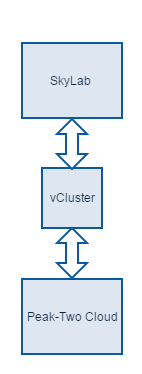
\includegraphics[width=92px,height=224px]{./images/system_architecture.png}	
		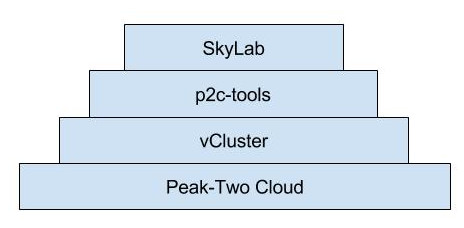
\includegraphics[scale=0.30]{./images/skylab_layers.jpg}			
		\caption{\label{fig:sysarch}Layers on which SkyLab is built on.}	
	\end{figure}	


    \begin{figure*}[ht]
      \centering
      %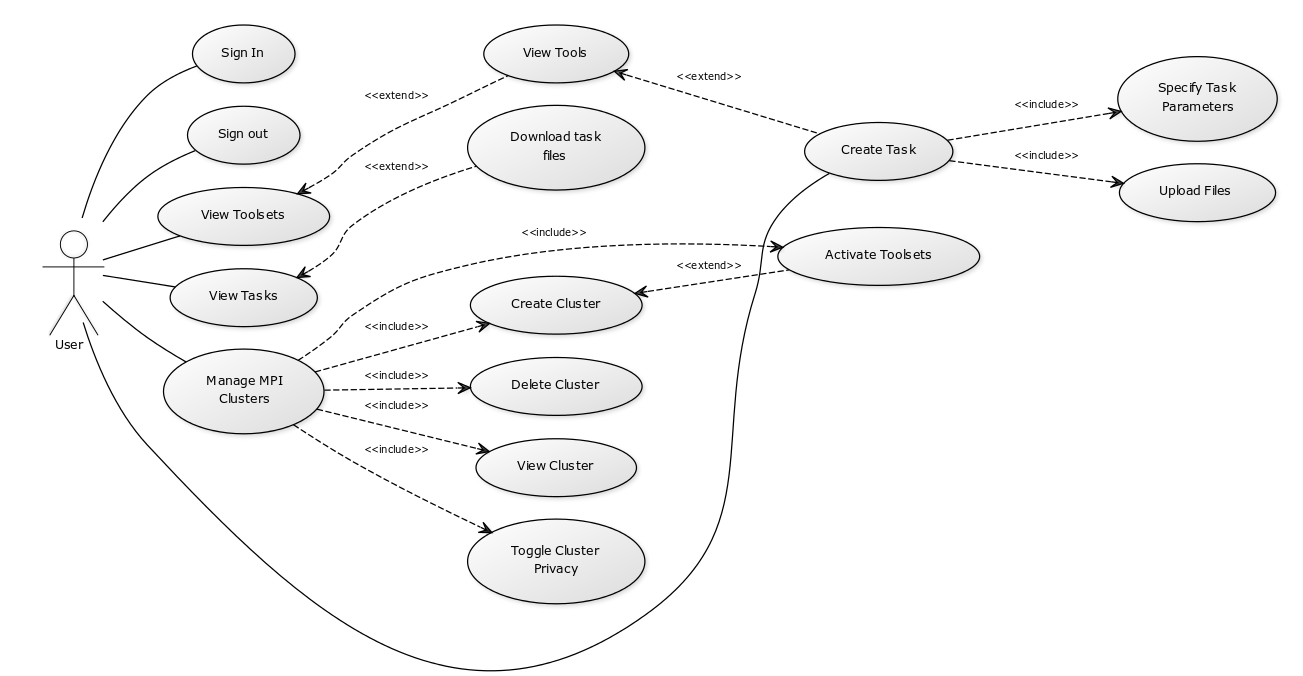
\includegraphics[width=500px,height=250px]{./images/use_case_large.png}
      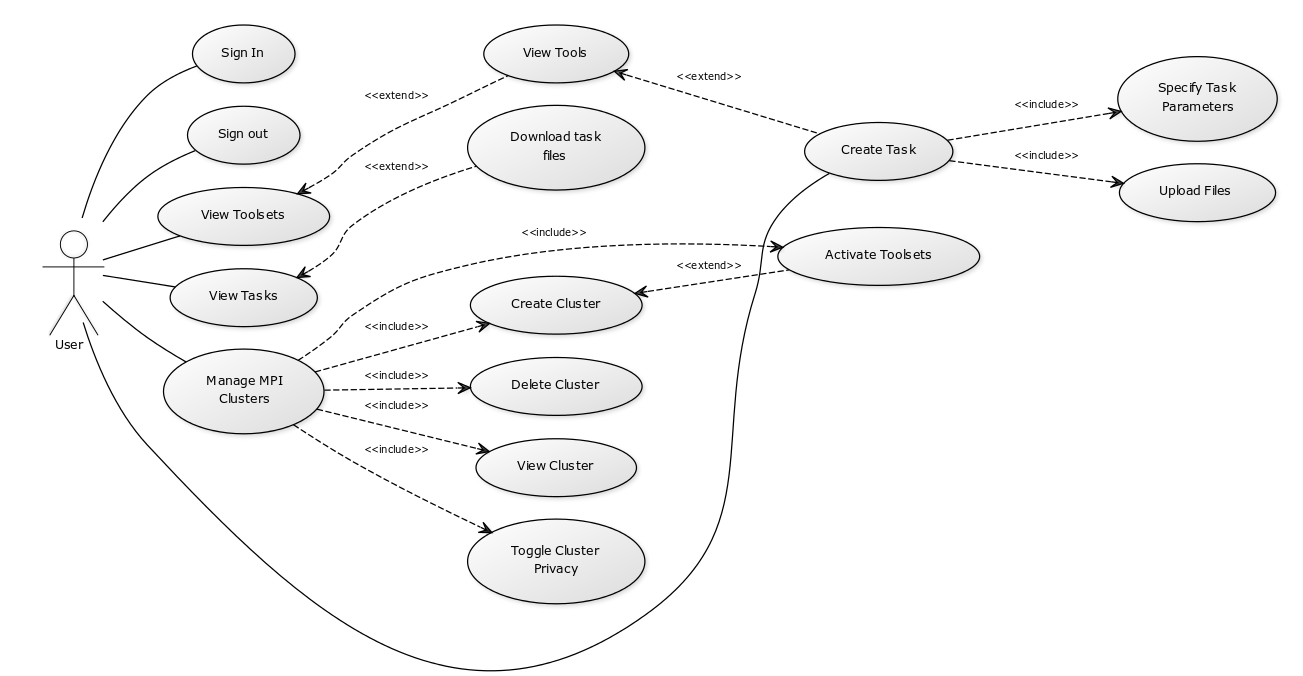
\includegraphics[scale=0.36]{./images/use_case_large.png}
      \caption{\label{fig:usecase}Use case diagram.}
    \end{figure*}

	\begin{figure*}[ht]
      \centering
      %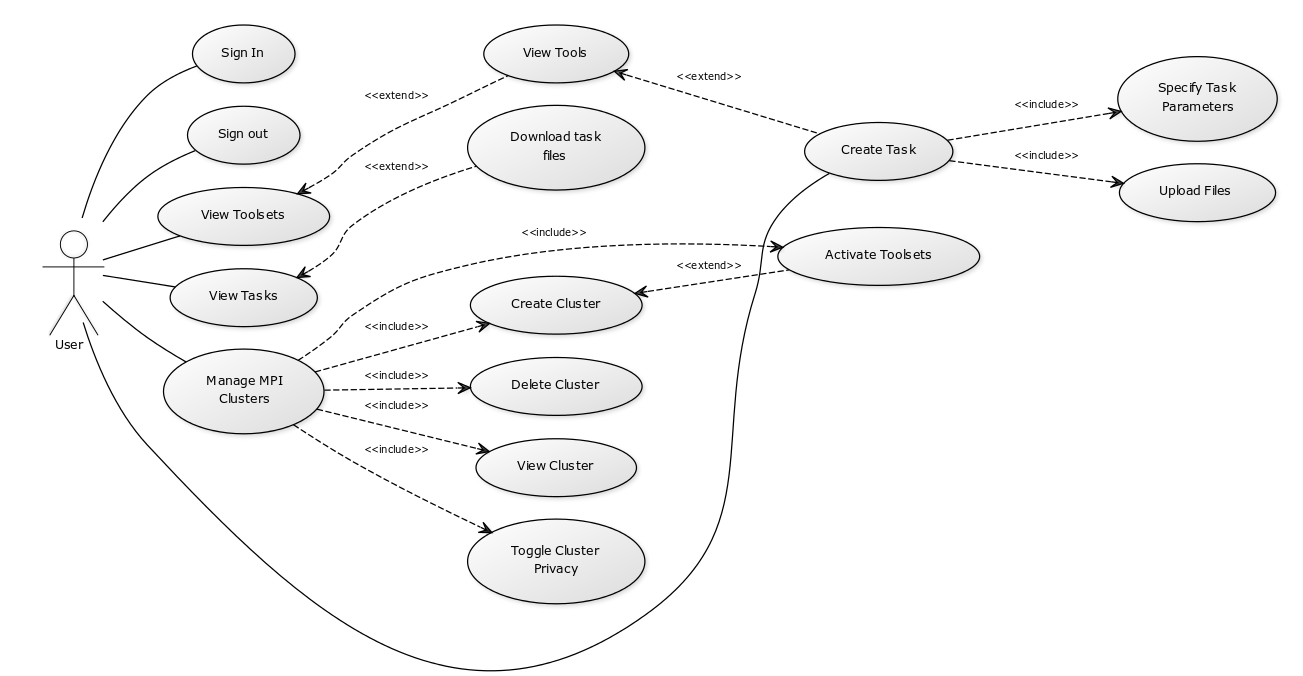
\includegraphics[width=500px,height=250px]{./images/use_case_large.png}
      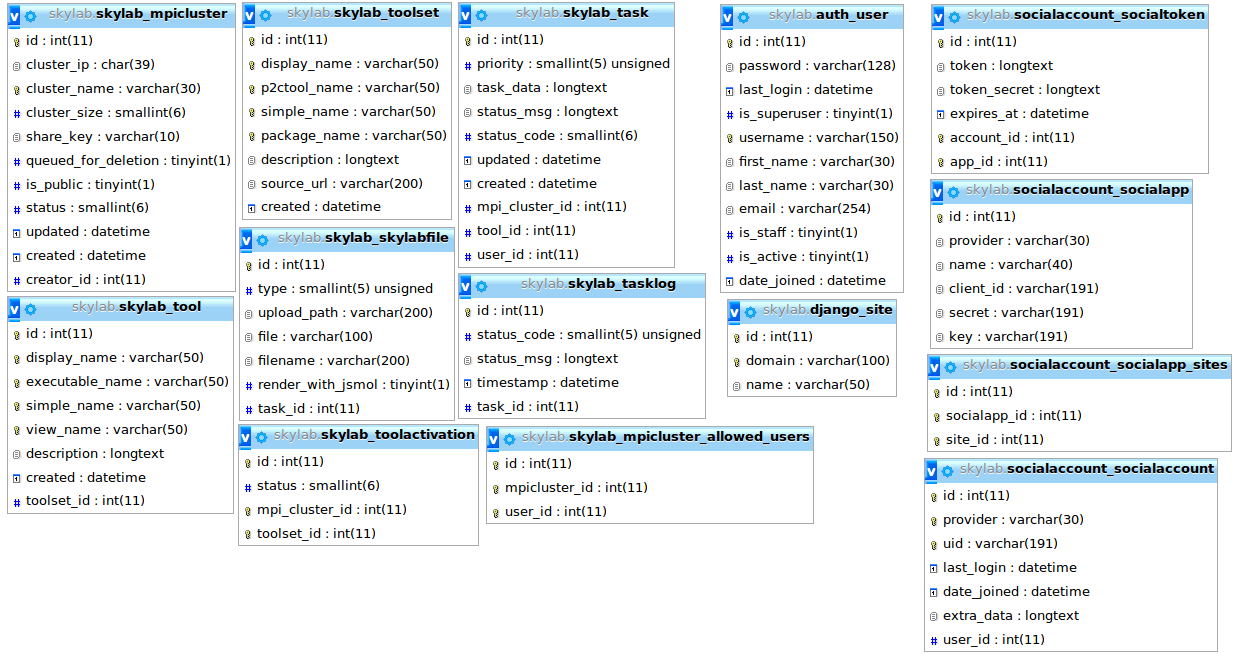
\includegraphics[scale=1.5]{./images/db_schema.png}
      \caption{\label{fig:dbschema}MariaDB database schema generated from Skylab's data models (see models.py).}
    \end{figure*}

\subsection{User Access}
Access to SkyLab is restricted to individuals with \textit{@up.edu.ph} email (hosted by Google) only. This is implemented  using the django-allauth\footnote{http://www.intenct.nl/projects/django-allauth/} package. Tables used with \textit{socialaccount\_} prefix, as shown in Figure ~\ref{fig:dbschema}, are used for authentication. Users logged in to this email can directly access SkyLab.

\subsection{Bootup}
SkyLab is deployed using the Apache Web Server via the \textit{mod\_wsgi} module. During bootup, toolsets are first loaded (by parsing the \textit{modules} directory) and logging is initialized. As a final step, an instance of \textit{MPIThreadManager} class is created. \textit{MPIThreadManager} (see bootskylab.py) is responsible for maintaining the connection to the node on which vCluster can be invoked. It opens a shell used to issue commands to the vCluster node and then creates an \textit{MPIThread} for each MPI cluster in the database. 

\subsection{MPI cluster management} 
An \textit{MPIThread}(see bootskylab.py) is spawned for each active cluster which handles the connection to the assigned cluster via Secure Shell (SSH). Creation and deletion of clusters is done by using \textit{vCluster} commands while tool activation is done by using \textit{p2c-tools}. The thread also manages task queuing and execution. Table \textit{skylab\_mpicluster} in Figure ~\ref{fig:dbschema} stores data on MPI clusters.
		
A cluster is either classified as public or private. If it is set to public, every user in the system can use it. On the other hand, for private clusters, the cluster will only be visible to the owner. The owner has the option to share the cluster to other users via the share key generated for the said cluster. 		

\subsection{Toolsets} 
As described in the Bootup section, the system searches for packages inside the \textit{modules} directory and load them at bootup. The toolsets will then be available for use with the system. The package must have a module named \textit{install.py} which contains function calls for integrating the package to  SkyLab. The package must also contain the corresponding \textit{views} and \textit{executable} classes for each tool. Tables \textit{skylab\_toolset} and  \textit{skylab\_tool} in Figure ~\ref{fig:dbschema} stores data for the tools.

All tool classes must inherit from the \textit{P2CToolGeneric} class (see basetool.py) and override the following methods to handle tool specific operations. 

\begin{itemize}
	\item \textit{test\_ssh\_connection} - Tests the SSH connection to the MPI cluster hosting the tool.
	\item \textit{sftp\_file\_transfer\_callback} - Callback method after an sftp operation. sftp is used to transfer files to and from a cluster.
	\item \textit{clear\_or\_create\_dirs} - Create task directories on the cluster.
	\item \textit{run\_commands} - Invoke the tool specific commands on the cluster. Must be overridden.
	\item \textit{handle\_input\_files} - Process the input files for the tool. Must be overridden.
	\item \textit{run\_tool} - Method that gets executed in a task. Must be overridden. Listing 1 shows an example implementation.
	\item \textit{handle\_output\_files} - Process output files. Must be overridden.
\end{itemize}

\begin{lstlisting}[label=runtool, language=Python, frame=single, caption=run\_tool method implementation for GAMESS.]
def run_tool(self, **kwargs):
    self.task.change_status
    	(status_msg='Task started',
    	status_code=150)
    self.clear_or_create_dirs
    	(task_remote_subdirs=
    	['input', 'output'])
    self.handle_input_files()
    self.run_commands()
    self.handle_output_files()
\end{lstlisting}


\subsection{Tasks} 
The system creates a task object for each task input by the user. A signal will then be sent and it is then received by the corresponding \textit{MPIThread} which queues the task for execution. When a task is executed, it calls the assigned executable class with the given parameters. On connection error, the task waits using exponential backoff before retrying. If the server crashes while running task execution, the task is just restarted. Table \textit{skylab\_task}  in Figure ~\ref{fig:dbschema} stores data for the tasks.				
		
Default task execution flow via the executable class is as follows:			
	\begin{enumerate}
		\item  Needed remote and local directories for execution are cleared or created.
		\item  Input files are uploaded to cluster.
		\item  List of commands given are executed.
		\item  Output files are sent back to the server.
		\item  Remote task folder is deleted.
		\item  Output files are served by the server.
	\end{enumerate}	

\subsection{Output Files}
Tools generate output files that must be returned to the user. Since SkyLab can support many tools, it handles output files differently for each tool. Modules must implement the \textit{handle\_output\_files} method of the \textit{P2CToolGeneric} class which is the super class of modules. This method's implementation typically downloads output files from the cluster running the tool to SkyLab's \textit{output} directory using sftp. If a tool has multiple output files, these are zipped first before downloading. The user will then be given links to download the output files. For modules like GAMESS, the ouput can be directly rendered on the browser (Figure ~\ref{fig:jsmol}).
	
\section{Results}
Figures ~\ref{fig:mpicreate} to ~\ref{fig:jsmol} show some of the screenshots that realize the use case (Figure ~\ref{fig:usecase}) for SkyLab. The screenshots were obtained from a SkyLab instance that is hosted on P2C itself.

		
\begin{figure}			
	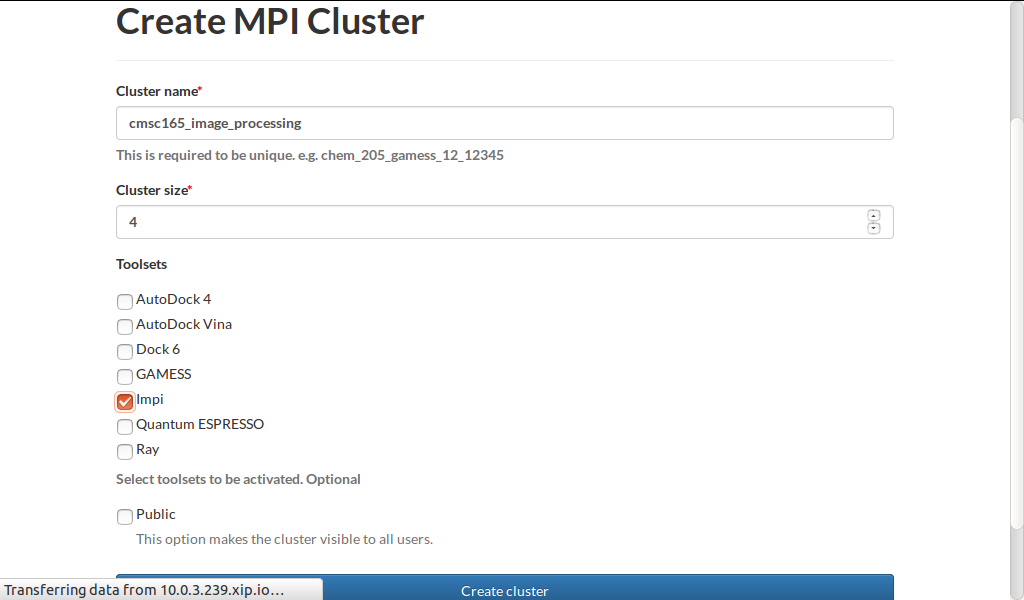
\includegraphics[scale=0.93]{./images/n_create_cluster_impi_printed.png}
	\caption{\label{fig:mpicreate}MPI cluster creation. A cluster named \textit{cmsc165\_image\_processing} is being created with the \textit{Impi} tool checked to be activated.}			
\end{figure}	
	
\begin{figure}			
	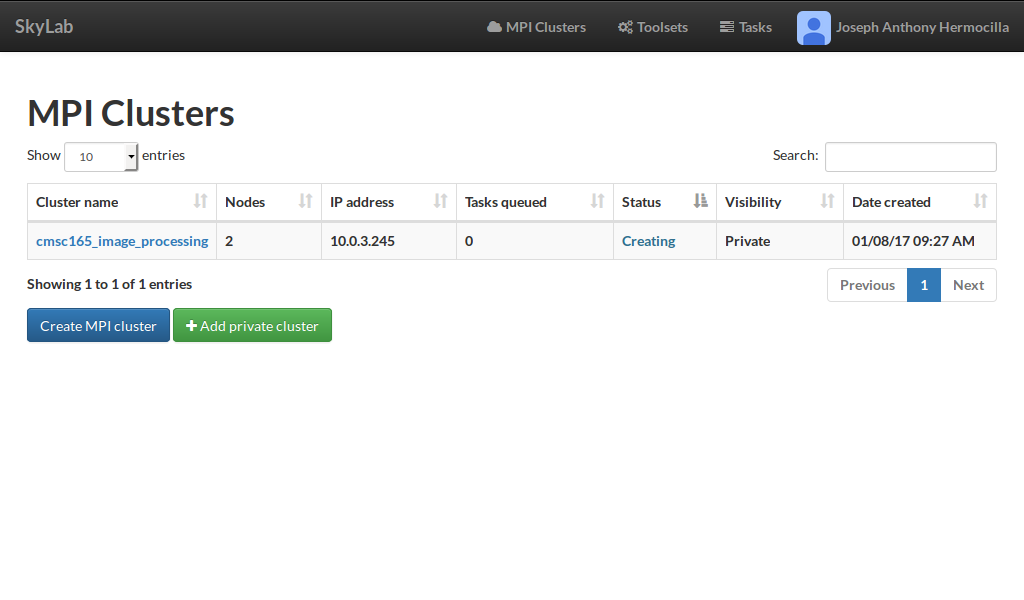
\includegraphics{./images/n_active_cluster_printed.png}
	\captionof{figure}{MPI cluster table. Currently deployed MPI clusters are shown with some of their properties such as IP address and creation timestamp.}		
\end{figure}
		
\begin{figure}			
	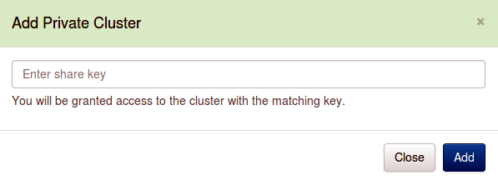
\includegraphics[scale=0.50]{./images/add_private_cluster_2.png}		
	\captionof{figure}{Set cluster visibility. A user can make a private cluster visible by entering a valid shared key.}			
\end{figure}	
		
\begin{figure}			
	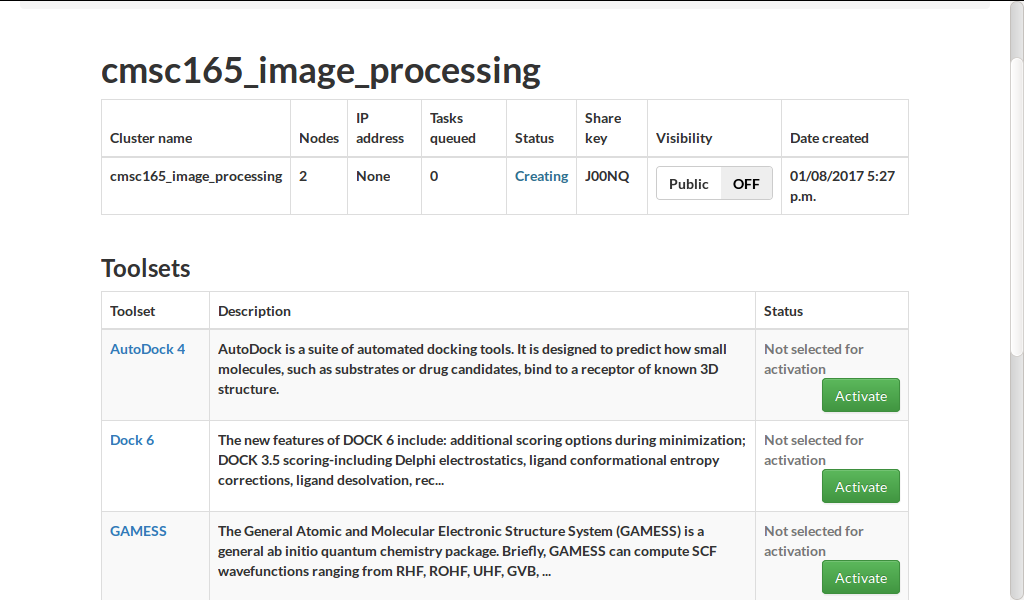
\includegraphics{./images/n_new_cluster_created_printed}
	\captionof{figure}{MPI cluster details view. The detailed view of the \textit{cmsc165\_image\_processing} MPI cluster with a list of tools that can be activated.}			
\end{figure}	
		
\begin{figure}			
	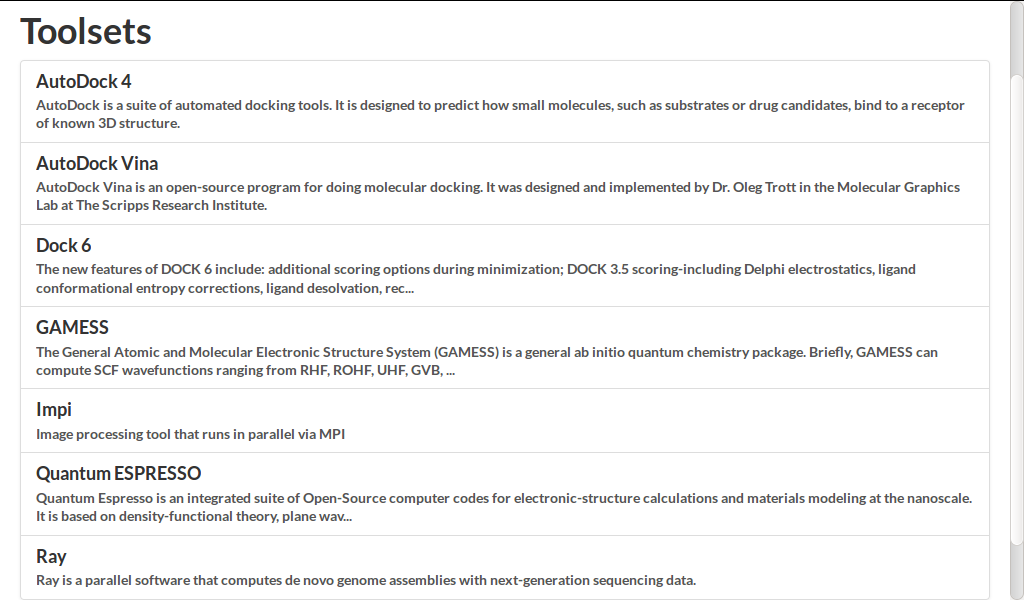
\includegraphics[scale=0.93]{./images/n_toolsets_printed.png}			
	\captionof{figure}{Toolset list view. The user can select from a list which tool to use.}	\end{figure}
		
\begin{figure}			
	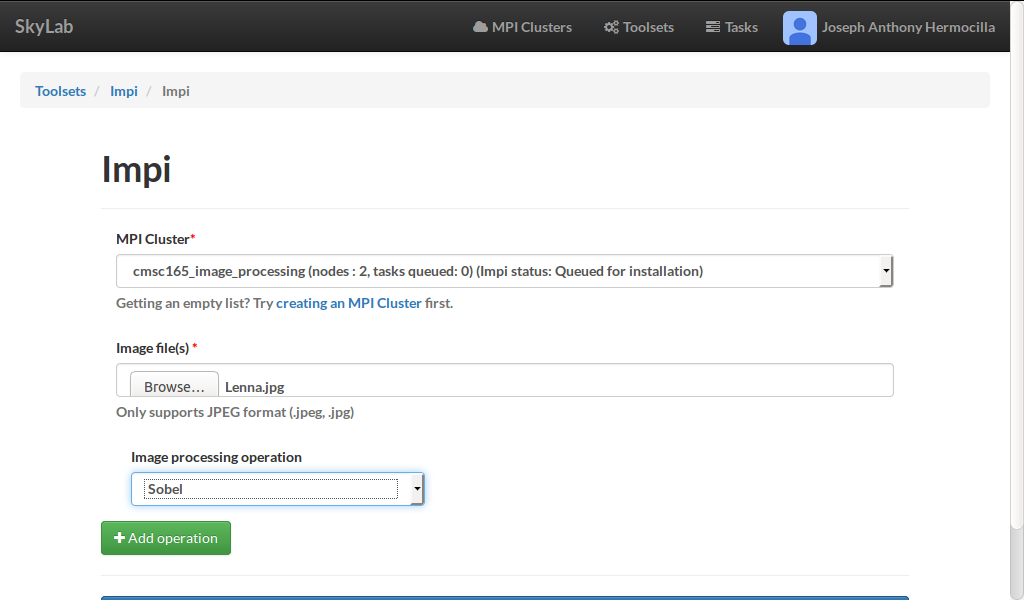
\includegraphics[scale=0.93]{./images/n_impi_parameters_printed.png}
	\captionof{figure}{Impi task creation form. The user will run an Impi task (sobel edge detection) with Lenna.jpg as input.}			
\end{figure}	
		
\begin{figure}			
	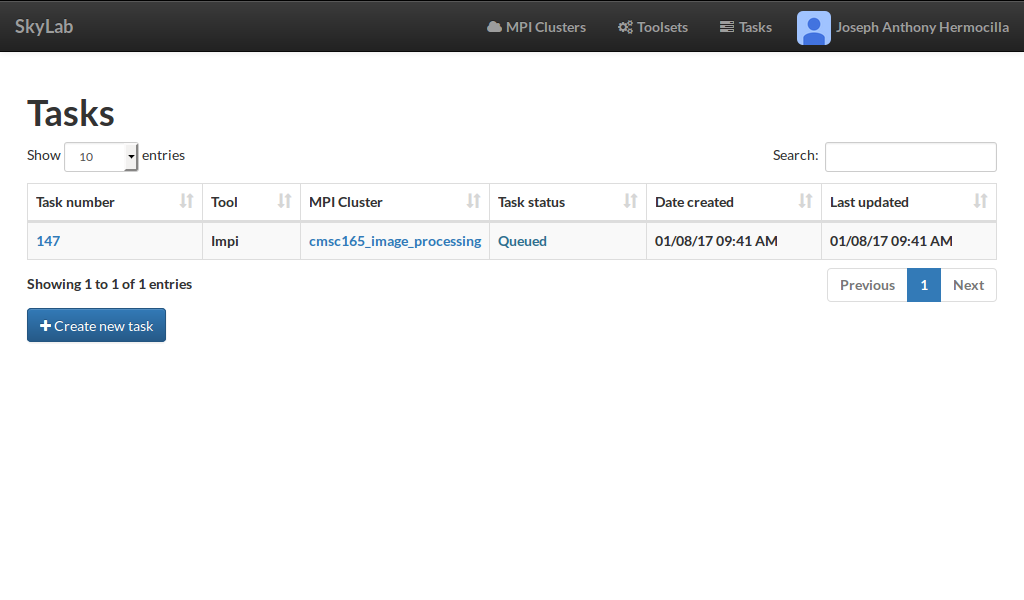
\includegraphics[scale=0.93]{./images/n_tasks_printed.png}			
	\captionof{figure}{Task table view. Impi task on the cmsc165\_image\_processing cluster is  currently queued for execution.}			
\end{figure}	

\begin{figure}			
	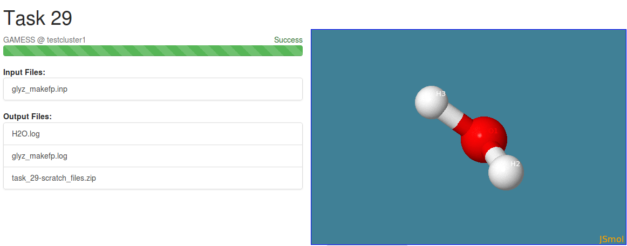
\includegraphics[scale=0.35]{./images/jsmol_detail_view_2.png}			
	\caption{\label{fig:jsmol}Task detail view.  JSmol \cite{IJCH:IJCH201300024} renders the compatible output files from a GAMESS task.}			
\end{figure}	
	
	
\section{Evaluation}
%	\begin{center}			
%			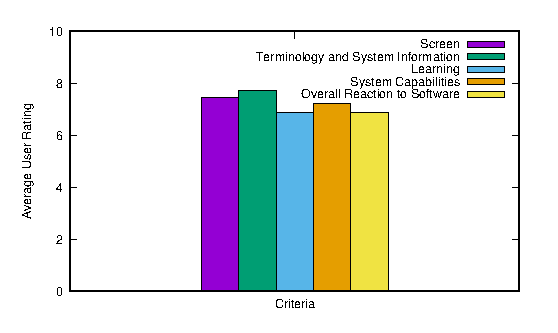
\includegraphics{./images/rating.eps}			
%			\captionof{figure}{Results of QUIS for SkyLab}			
%	\end{center}

\begin{figure}			
	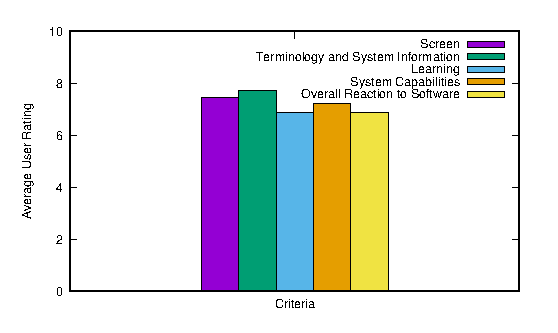
\includegraphics[scale=1.0]{./images/rating.eps}			
	\caption{\label{fig:quis}Results of QUIS for SkyLab}			
\end{figure}


	The system has been evaluated by 56 respondents by answering a survey based on Questionnaire for User Interface Satisfaction (QUIS) \cite{chin1988development}. The respondents are students who are unfamiliar with both HPC tools and the concept of MPI systems.  They are asked to test features of SkyLab by following a set of instructions and using input files provided. On the average, the users rated their overall experience with SkyLab to 6.9/10. The users listed the simplicity of the user interface to be the most positive aspect of the system while the slow speed of task processing is said to be the most negative. Majority of the tools supported by SkyLab have inherently long processing time which is not known to the respondents. The system does not focus on optimizing the said tools to achieve better performance but rather it focuses on simplifying the user's task submission process. 

\section{Related Work}
Traditional usage of HPC applications requires users to learn job submission systems like Torque\footnote{http://www.adaptivecomputing.com/products/open-source/torque/} or Slurm \footnote{https://slurm.schedmd.com/} that are used via the command line. Scientific workflow systems make it easier for users to use their tools without mastering the command line.

The main motivation for developing SkyLab is Yabi\cite{7411021620120101}. It provides a web interface with support for workflow environments with focus on introducing HPC applications to non-technical audience. Users can create and reuse workflows, and manage large amounts of data while system administrators can configure tools via the web interface as well. It is currently in use by multiple institutions, and is maintained as an open-source project.	    	    
	    
Another related project is Web Interface for mpiBLAST (WImpiBLAST). It supports mpiBLAST, a parallel implementation of Basic Local Alignment Search Tool (BLAST). BLAST is a software used for sequence homology similarity search in large databases of gene sequences. mpiBLAST can utilize HPC clusters to achieve faster computing speeds but it requires knowledge in using MPI commands to benefit from its advantages. WImpiBLAST addresses this problem by providing the user a web interface to simplify the steps to use mpiBLAST\cite{9686120720140601}.   
	
Pegasus \cite{deelman2005pegasus} is another scientific workflow system that allows users to specify workflows at an abstract level. This tool is particularly useful in grid computing with a lot of distributed resources.

The Kepler \cite{ludascher2006scientific} system supports low-level workflows for grid engineers at the same time analytical knowledge discovery workflow for scientists.	

Taverna \cite{hull2006taverna} is currently gaining popularity as a modern domain-independent workflow management system. It is written in Java and has moved to the Apache Software Foundation incubator project\footnote{https://taverna.incubator.apache.org/}. It allows scientists to construct complex analysis given limited background in computing.  
	
\section{Conclusion and Future Work}
SkyLab allowed users to manage MPI clusters and submit tasks without the need for technical expertise in command line and scripting. This makes the advantages of HPC available to non-technical users. This is achieved by parsing form inputs to generate commands for task execution. Task files can be download from the server and output files are displayed with the help of JSmol. The system is also configured to install tool sets found in the modules folder making it possible to accommodate additional tools. Based on the user acceptance test conducted, the users found the system to be acceptable in terms of the criteria provided, in general. 

SkyLab achieved its main objectives but its features can still be improved and additional features can be introduced. Improved input parameter checking and error handling will make the system more robust. There are still use cases of tools that are yet to be supported. Input file generation can make the process more interactive and more customizable.  Workflow design support will enable users to run complex tasks. Support for custom MPI programs will make it easier for developers to utilize the system as a test environment. Task scheduling and resource management algorithms can be used to efficiently handle resource-intensive or time consuming tasks. For example, a cluster can borrow resources from idle clusters. These recommendations will provide the users a better experience in using the system for academic and research purposes. 

% APPENDICES
%\appendices

%\section{Proof of the First Zonklar Equation}
%Appendix one text goes here...

%\section{}
%Appendix two (without title) text goes here...

% ACKNOWLEDGMENT
\section*{Acknowledgment}
This work is supported by the Philippine Department of Science and Technology Accelerated Science and Technology Human Resource Development Program. We also would like to thank our collaborators who provided the use cases for the tools: Dr. Abraham Padama (Material Science), Dr. Marlon Manalo (Chemistry), and Prof. Arian Jacildo (Bioinformatics). Finally we acknowledge the valuable comments by the reviewers.
%Many thanks to...
% BIBLIOGRAPHY
% \nocite{*}

% BIOGRAPHY
%\begin{biography}[{
\includegraphics{./yourPicture.eps}}]{Student M. Name}
%Biography text here...
%\end{biography}



